A diferencia de la mayoría de los métodos de imagen, basados en la absorbancia o reflectancia de ondas electromagnéticas como los Rayos X, la resonancia magnética se basa en principios físicos y matemáticos que pueden ser intimidantes de inicio. Mientras que en otros métodos la imagen es obtenida casi directamente, las imágenes por resonancia magnética son construidas a partir de la decodificación de múltiples señales. Sin embargo, una vez que son comprendidas ponen de manifiesto la enorme inventividad del ser humano al llevar tan altos niveles de abstracción a algo tan útil como lo es la generación de imágenes del cuerpo humano. Pocas técnicas reúnen tantos conceptos en áreas tan diversas como la física clásica y cuántica, las matemáticas, el proceso de señales y la estadística, como lo hace la imagenología por resonancia.

Comprender a fondo la manera en que se generan las imágenes de resonancia no es trivial, y requiere conocer los fundamentos de las diversas áreas que se reúnen en esta metodología. Todos los conceptos están inevitablemente encadenados y poseen un grado de complejidad jerárquica. A pesar de esto, existe una gran ventaja: en innumerables ocasiones los conceptos avanzados ayudan a afianzar los conocimientos de los conceptos que les preceden. Debemos notar que sería muy difícil, si no imposible, aprender los conceptos avanzados teniendo unas bases débiles, pero no es raro que el estudiante de resonancia magnética pueda imaginar cada vez mejor los fundamentos conforme avanza en su estudio.

Iniciaremos nuestro recorrido por la resonancia magnética dando una vista a vuelo de pájaro sobre los conceptos que participan en la generación de imagen, desde el nivel atómico hasta la visualización de la misma. La intención es proveer una visión global sobre la manera en que los conceptos se encadenan, señalando únicamente los principios fundamentales. Para quien se inicia en resonancia magnética, este capítulo pretende servir como brújula, y es labor de los siguientes capítulos de la Parte \ref{part_principiosBasicos} de este libro, el llenar los huecos y ofrecer más detalles. 


\section{Fenómeno de resonancia magnética nuclear}
Todos los átomos con un número impar de protones y/o neutrones en su núcleo poseen un spin distinto de cero. Estos núcleos se comportan como pequeñísimos imanes, con sus respectivos polos Norte y Sur. Estos imanes no se encuentran inmóviles, sino que se encuentran rotando (como lo hace nuestro planeta), y la velocidad a la que rotan (su frecuencia) es dependiente del campo magnético que están experimentando. Más correctamente, los átomos experimentan un movimiento de precesión \index{precesión} en torno a la orientación del campo magnético local (Figura \ref{fig:spins}, A), cuya frecuencia es dependiente del mismo. Si el átomo está flotando en un medio con un campo magnético bajo, precesará a una frecuencia baja; si está inmerso en un campo magnético poderoso, precesará a una alta frecuencia. A esta relación se le conoce como la frecuencia de Larmour y es explorada en más detalle en el Capítulo \ref{chapter_fenomeno}. Sin embargo, no todos los átomos precesan a la misma frecuencia estando en el mismo campo magnético. Cada especie atómica tiene una ``firma'', una frecuencia a la que precesa dependiendo del campo magnético, y que la distingue de todas las otras especies atómicas. Esta firma se conoce como la constante giromagnética \index{constante giromagnética} y se simboliza con la letra $\gamma$. Por ejemplo, la constante giromagnética del hidrógeno es alrededor de 42.5 MHz/T, lo que nos dice que si un átomo de hidrógeno está en un campo magnético de un Tesla, dará 42.5 millones de vueltas en un segundo. Si ahora ponemos ese átomo en un campo magnético de 3 Teslas, precesará a una frecuencia de 127.5 MHz. Como el hidrógeno es el elemento más abundante en los seres vivos, es el átomo explotado para la realización de imágenes por resonancia magnética \footnote{No es el único, habiendo ejemplos notables de imagen utilizando el sodio.}. Habiendo solamente un protón en el núcleo del hidrógeno, en la mayoría de los textos de resonancia magnética, y en este en particular, es frecuente la utilización indistinta de los términos ``núcleo'', ``protón'' y ``spin'' para referirse al núcleo del átomo de hidrógeno.

\begin{figure}[htb]
 \centering
 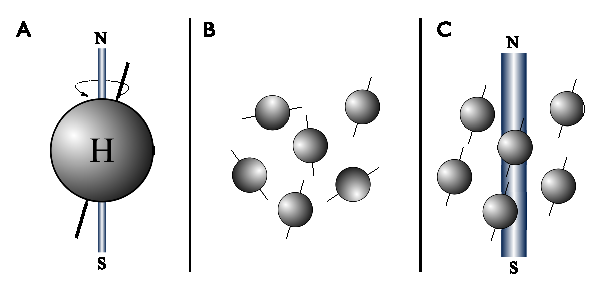
\includegraphics{spins}
 \caption{Los spins se orientan de acuerdo al campo magnético que experimentan y precesan alrededor de él (A). En el caso de un campo magnético poco potente, los spins estarán orientados aleatoriamente (B), mientras que si experimentan un campo magnético de gran intensidad, se alinearán acordemente (C).}
 \label{fig:spins}
\end{figure}



Imaginemos ahora un sencillo escenario: disponemos de una muestra de agua pura sobre una mesa cualquiera. Si analizáramos la orientación de los polos magnéticos de todos los núcleos de hidrógeno que tenemos, éstos apuntarían en diversas direcciones. Facilita la visualización si imaginamos pequeños imanes de barra orientados aleatoriamente (Figura \ref{fig:spins}, B). Si ahora colocamos nuestra muestra dentro de un campo magnético potente y analizamos nuevamente sus orientaciones, veremos que ahora todos estos imanes de barra apuntan en la misma dirección (Figura \ref{fig:spins}, C). Si recordamos que las brújulas apuntan hacia el Norte, a menos que las pongamos frente a un campo magnético aun más potente que el terrestre \footnote{1 Tesla = 10 000 Gauss. El campo magnético terrestre es de solamente 0.5 Gauss.}, no resulta soprendente que ahora todos estos imanes de barra apunten en la dirección del campo magnético que ahora experimentan. No solamente apuntan en la misma dirección, sino que también todos precesan a la misma frecuencia al estar todos experimentando el mismo campo magnético. Ahora, prendamos un campo magnético adicional pero, a diferencia del primero, éste está dando vueltas alrededor de nuestra muestra a la misma frecuencia que la que están precesando los spins (frecuencia de Larmour). Esto en la práctica es una radiofrecuencia.  Ahora nuestros pequeños imanes tienen un nuevo lugar a donde voltear y, a pesar de que este nuevo campo magnético en rotación es más débil que el primero, les resulta más atractivo, porque precesa a la misma frecuencia que ellos. Si hemos hecho que nuestro campo magnético rotatorio (radiofrecuencia) gire en un plano transversal al campo magnético principal, nuestros spins ahora querrán voltearse sobre este plano, efectivamente desviándose de la orientación del campo magnético principal. Qué tanto logren este cometido dependerá de qué tanto tiempo dejemos prendida nuestra radiofrecuencia. Además, en cuanto apaguemos nuestra radiofrecuencia, los spins ahora solo verán el campo magnético principal y regresarán a alinearse con él. Durante esta realineación los spins emitirán de regreso el exceso de energía que absorbieron de la radiofrecuencia, y lo harán a la misma frecuencia. De aquí el nombre de \emph{resonancia}, y ya hemos visto de donde provienen los términos \emph{magnética} y \emph{nuclear} (si bien en general se evita decir esta última palabra para evitar pensar en fenómenos de radiación). Este fenómeno que acabamos de describir es la base que permite la espectroscopía e imagenología por resonancia magnética, pero hace falta saber cómo explotarlo para poder traducirlo.



\section{Codificación espacial}
\label{sec_codificacionEspacial}
Hemos recibido una señal que nos han regresado las moléculas de agua de nuestra muestra gracias al fenómeno de resonancia magnética. Por supuesto que la magnitud de esta señal irá en relación directa con la cantidad de átomos de hidrógeno, y con esto tenemos una manera muy complicada y costosa para medir cuánta agua hay en nuestra muestra. Si bien en el caso de agua el ejercicio sería ridículo, este es el principio que rige la espectroscopía, que logra medir la concentración de diversas moléculas en una mezcla (Capítulo \ref{chapter_espectro}). Pero notemos una gran ventaja que tenemos: la frecuencia de resonancia depende directamente del campo magnético que experimentan los spins. Hasta ahora habíamos puesto nuestra muestra en un campo magnético homogéneo, provocando que todos los spins resonaran a la misma frecuencia. ¿Qué pasará entonces si introducimos variaciones en la potencia del campo magnético que sean dependientes de su lugar en el espacio? Los spins precesarán a distinta frecuencia, las cuales nos informarían acerca de la potencia del campo magnético que están experimentando. Dado que nosotros hemos introducido la perturbación en el campo magnético, hemos logrado codificar la posición espacial de los spins, al menos en una dimensión (Figura \ref{fig:gradientesSimple}). Las bobinas (o imanes secundarios) llamados de gradiente son los responsables de sumar o restar la potencia del campo magnético principal, logrando variaciones en el orden de los mT/m (por ejemplo, un gradiente capaz de generar 40 mT/m, variará el campo magnético principal 4 mT a lo largo de 10 cm). La manera en que la segunda dimensión es codificada es similar, pero mediante el uso de la fase del spin (hacia dónde voltea el spin si lo vemos desde arriba) y es explicada en detalle en el Capítulo \ref{chapter_espacial}.

\begin{figure}[htb]
 \centering
 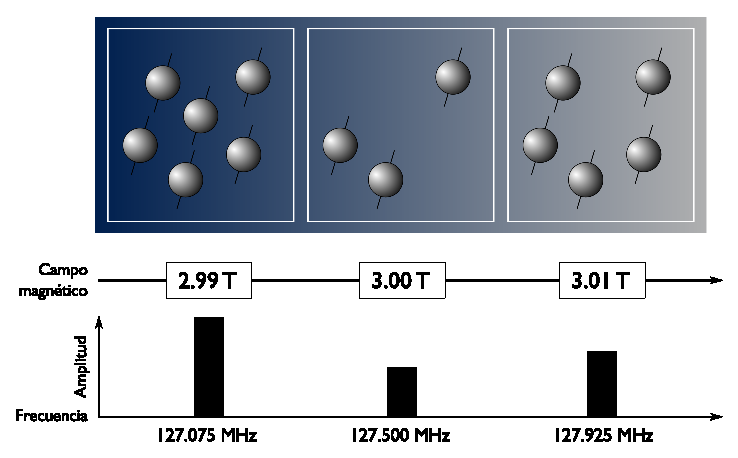
\includegraphics{gradientesSimple}
 \caption{Codificación espacial. Tres muestras, cada una con cantidades distintas de átomos de Hidrógeno, experimentan un campo magnético que aumenta en intensidad de izquierda a derecha. Cada muestra resonará a distinta frecuencia, y la amplitud de la misma dependerá de la cantidad de átomos que contiene.}
 \label{fig:gradientesSimple}
\end{figure}




\section{Secuencias de pulsos}

 Como hemos visto, los ingredientes para generar una imagen son los pulsos de radio-frecuencia y los gradientes del campo magnético y, aplicados en diversos momentos con duraciones específicas, logran imágenes con características específicas. La receta que utiliza estos ingredientes, en los tiempos y duraciones adecuadas, se denomina secuencia de pulsos. Suelen ser representadas mediante una línea de tiempo en la cual suceden los eventos, y los parámetros que las definen son precisamente los intervalos de tiempo entre ellos, o la intensidad de los mismos. Por ejemplo, el tiempo que transcurre entre dos excitaciones sucesivas de los spins se conoce como tiempo de repetición, o TR. La secuencia de pulsos para nuestro simple experimento de la Sección \ref{sec_codificacionEspacial} se ilustra en la Figura \ref{fig:secuenciaSimple}.

\begin{figure}[htb]
 \centering
 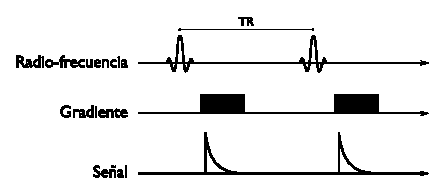
\includegraphics{secuenciaSimple}
 \caption{Secuencia de pulsos con codificación espacial en una sola dimensión (2 repeticiones).}
 \label{fig:secuenciaSimple}
\end{figure}




\fancybreak{* * *}


Con esta vista preliminar y caricaturesca, hemos logrado llevar el fenómeno de resonancia magnética hasta una imagen (al menos en una dimensión). Hemos obviado muchos detalles que contribuyen a la formación de la imagen, y no hemos tratado puntos esenciales como los fenómenos de relajación (Capítulo \ref{chapter_relajacion}), fundamentales para la existencia de contraste en una imagen. Mediante el uso juicioso de ingeniosas secuencias de pulsos, podemos hacer que los spins ``bailen el son que queramos``, lo que hace a la imagenología por resonancia magnética una de las técnicas mas poderosas y flexibles para la obtención de distintos tipos de información de una manera no invasiva (ver Parte \ref{part_protocolos}). El resto de los capítulos de la Parte \ref{part_principiosBasicos} brindan más información sobre aspectos específicos de estos interesantes temas.


% \bibliographystyle{concha2}
% % \bibliography{libroResonancia}
